\documentclass{beamer}
\usetheme{Warsaw}

\usepackage[utf8]{inputenc}
\usepackage{fancybox}
\usepackage{multimedia} 
\usepackage{subfig}
\usepackage{amsmath}

\usepackage[all]{xy}
\begin{document}


\title[Computergrafik] % (optional, only for long titles)
{Computergrafik

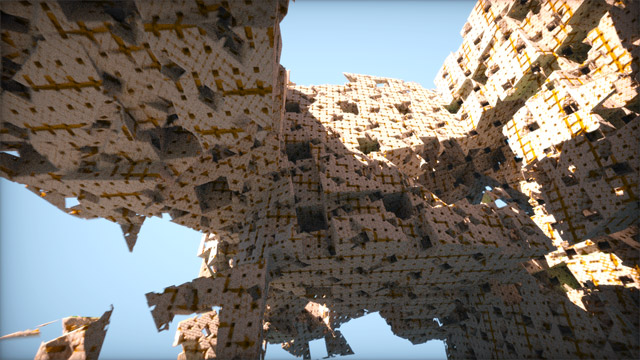
\includegraphics[scale=0.36]{images/cover}
}
\subtitle{}
\author[Dr. Johannes Riesterer] % (optional, for multiple authors)
{Dr.  rer. nat. Johannes Riesterer}

\date[KPT 2004] % (optional)
{}

\subject{Computergrafik}

\begin{frame}
    \frametitle{Perspektive}
\framesubtitle{}
\begin{center}
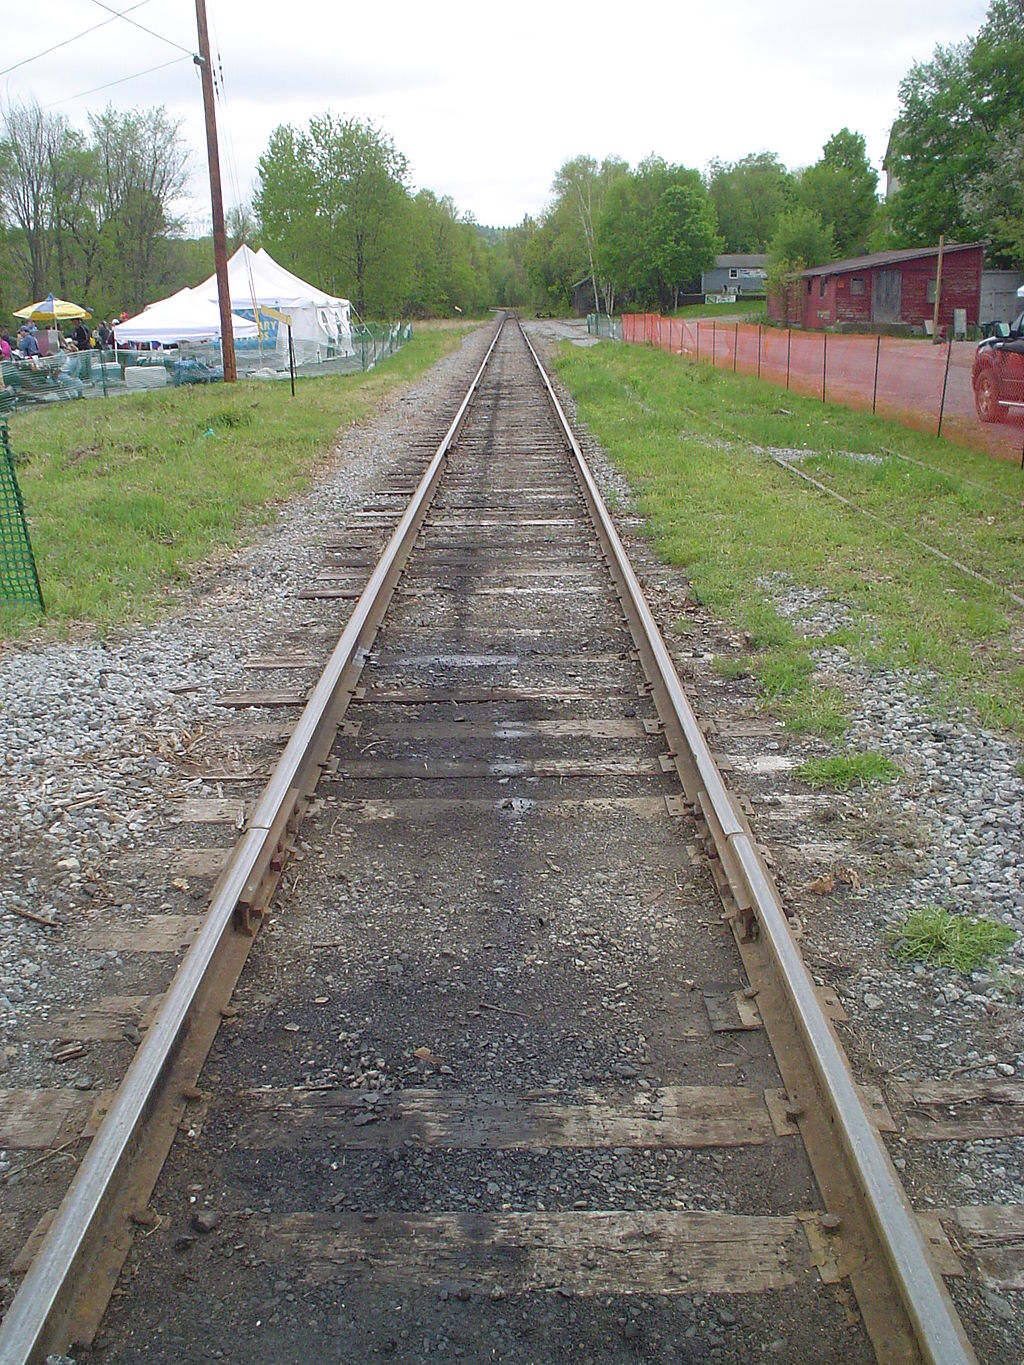
\includegraphics[scale=0.15]{images/Railroad}
\end{center}
\end{frame}


\begin{frame}
    \frametitle{Perspektive}
\framesubtitle{}
    \begin{block}{Projektionen}
\begin{center}

\includegraphics[scale=0.15]{images/projs}
\end{center}
\end{block}

\end{frame}



\begin{frame}
    \frametitle{Perspektive}
\framesubtitle{}
    \begin{block}{Orthogonale Projektion}
\begin{center}
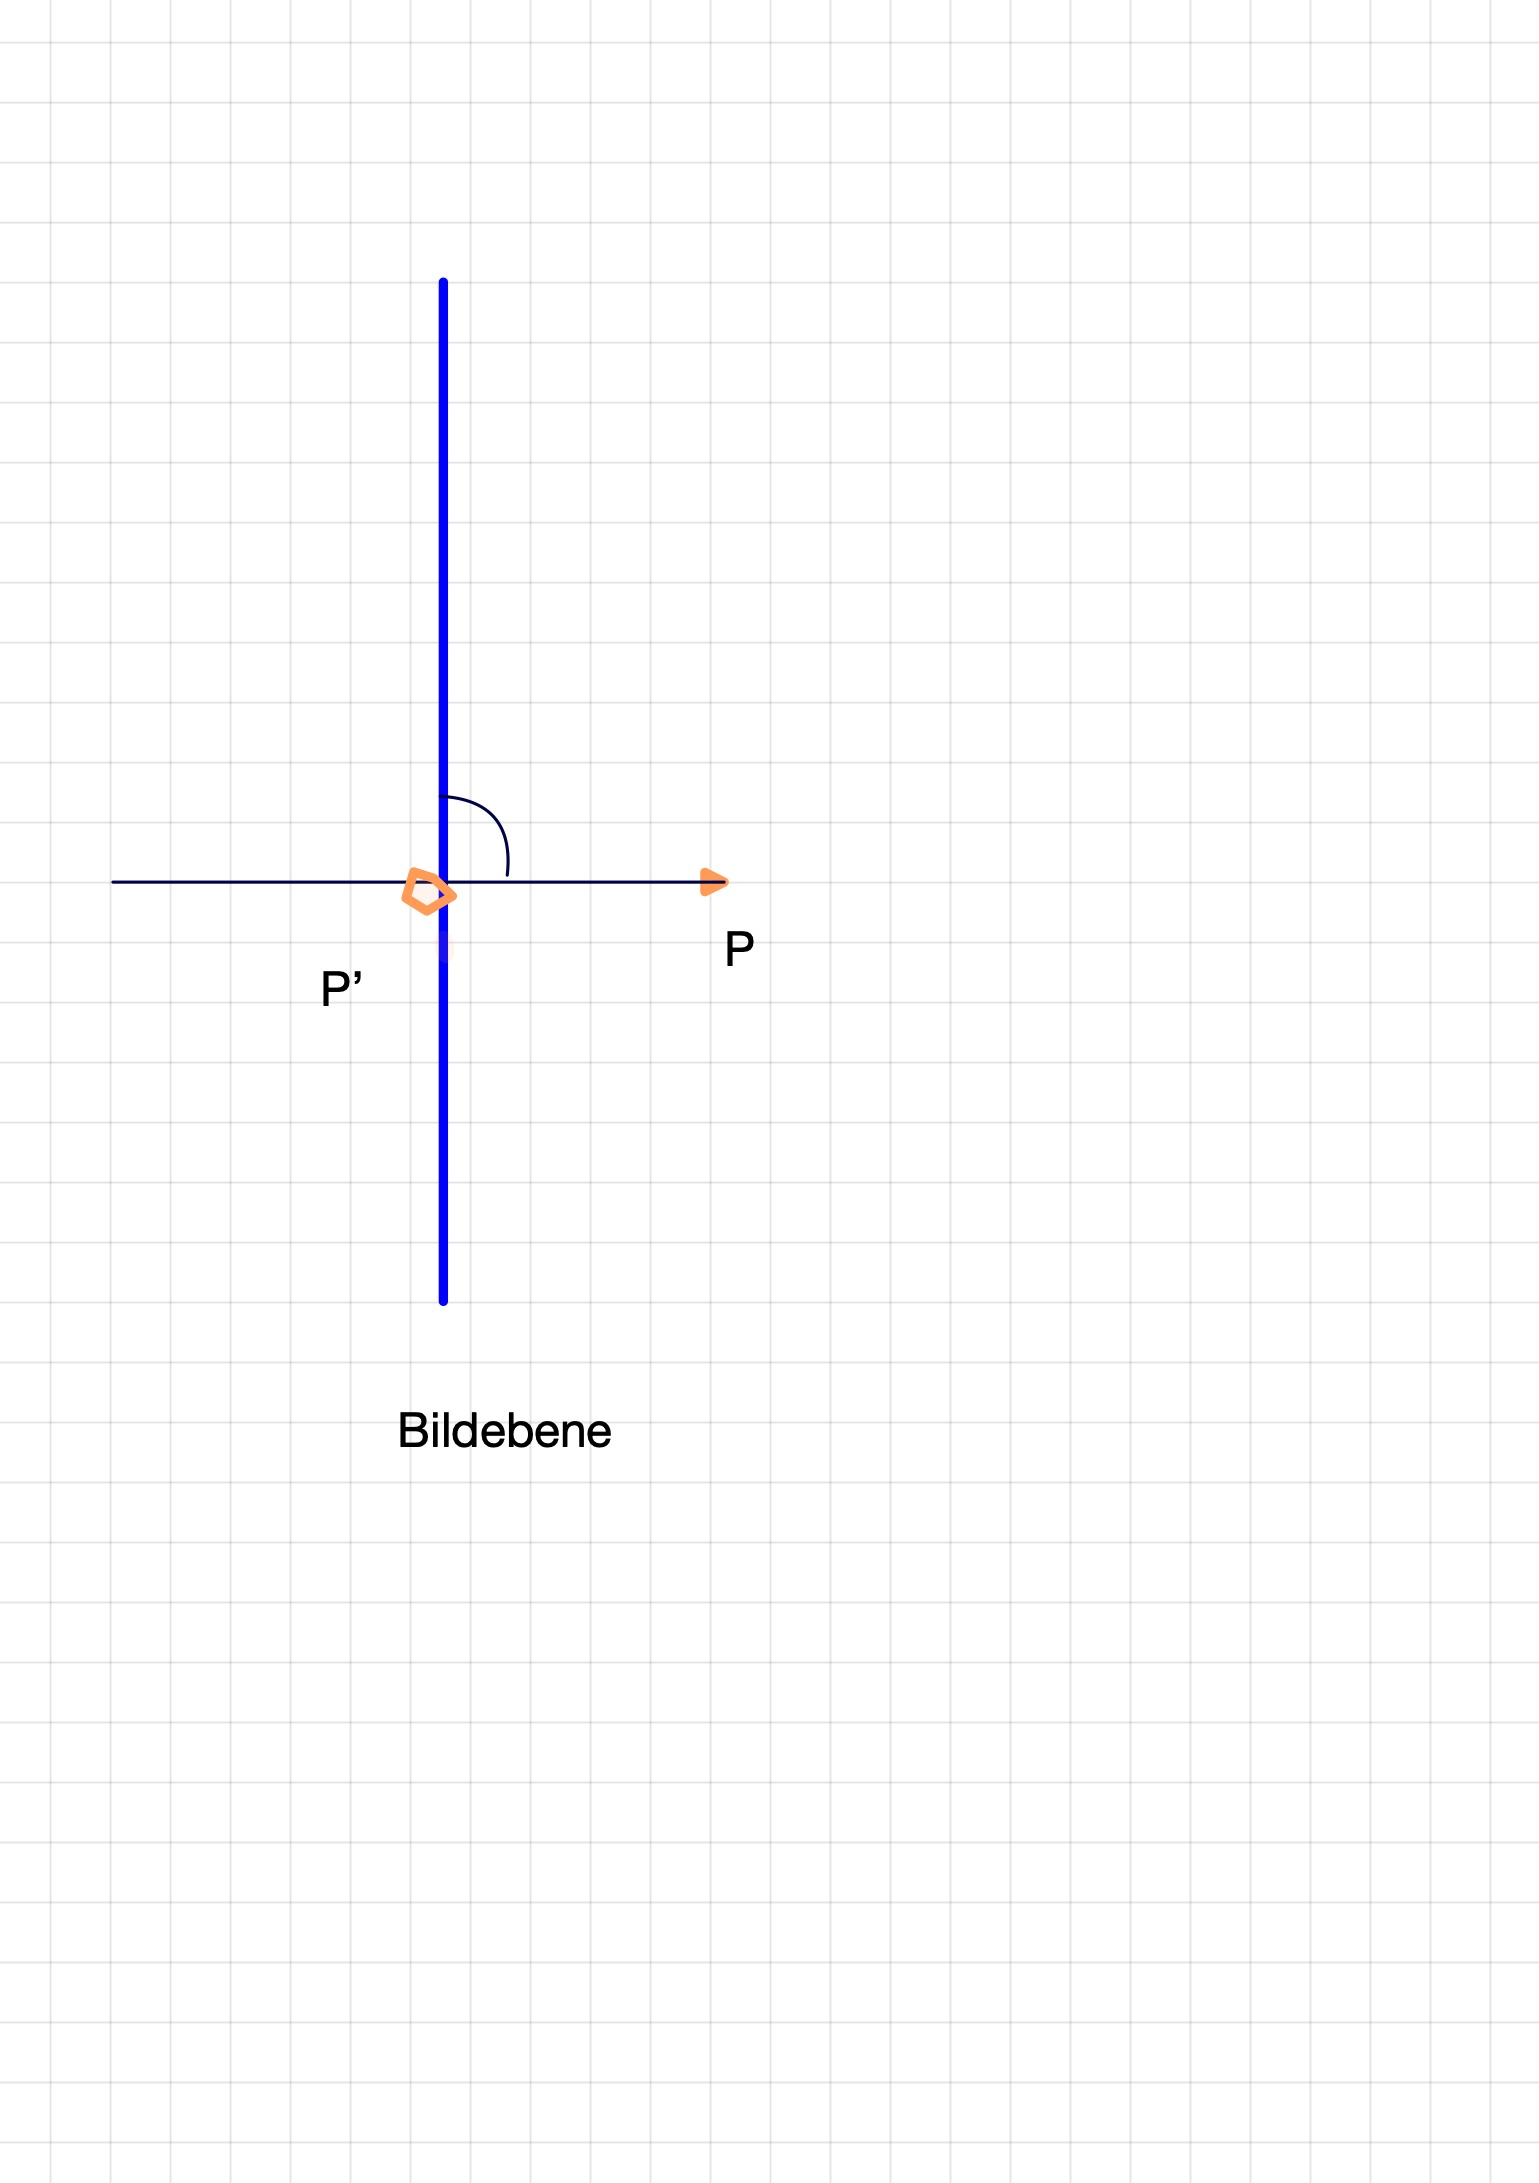
\includegraphics[scale=0.15]{images/oproj}
\end{center}
\end{block}

\end{frame}



\begin{frame}
    \frametitle{Perspektive}
\framesubtitle{}
    \begin{block}{Projektionen}
\begin{center}
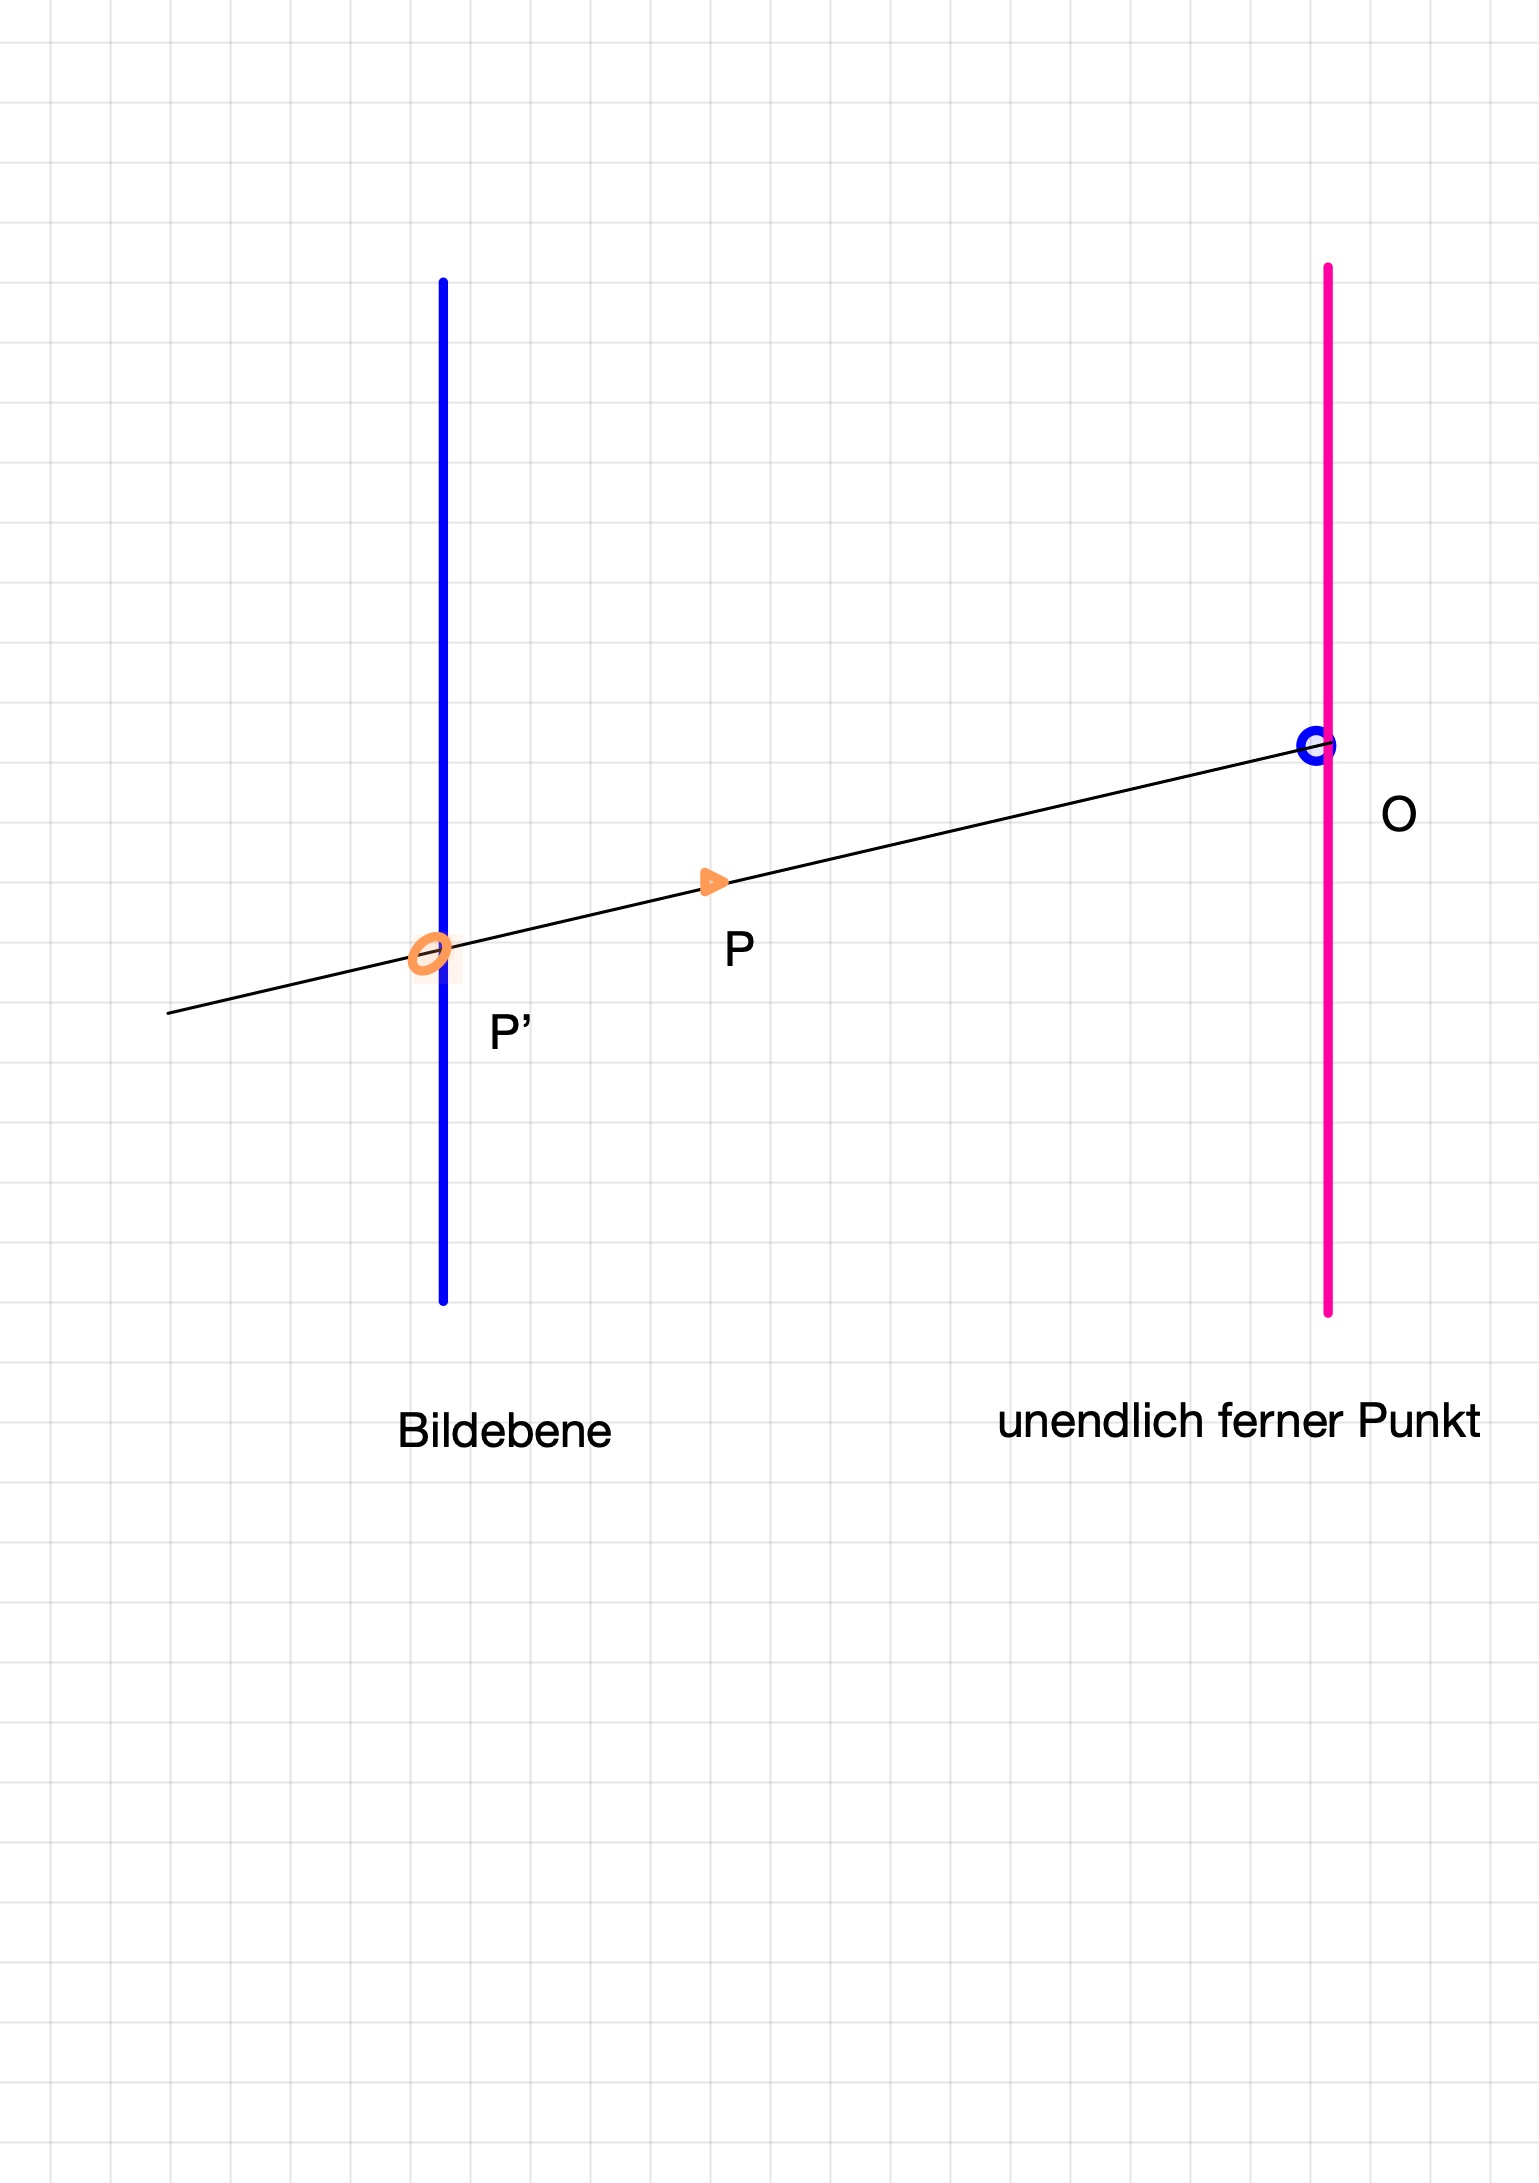
\includegraphics[scale=0.15]{images/proj1}
\end{center}
\end{block}

\end{frame}




\begin{frame}
    \frametitle{Perspektive}
\framesubtitle{}

\begin{center}
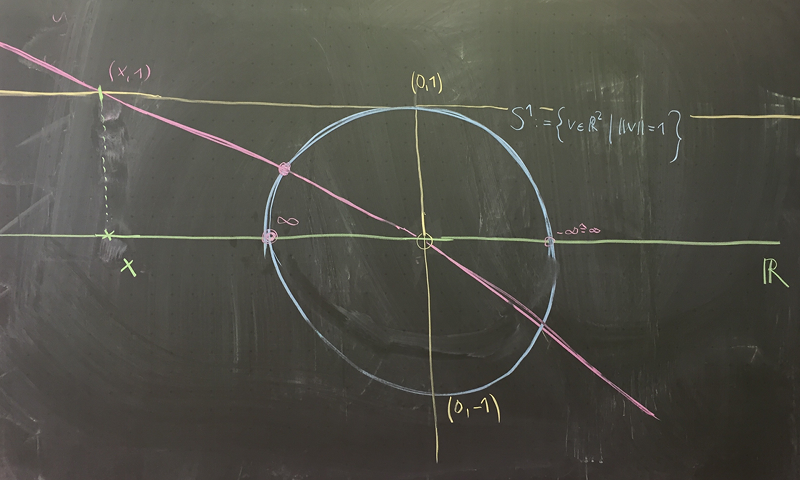
\includegraphics[scale=0.40]{images/proj2.png}
\end{center}
\end{frame}


\begin{frame}
    \frametitle{Perspektive}
\framesubtitle{}
\begin{block}{Projektier Raum}

Der projektive  Raum ist definiert als
\begin{align*}
\mathbb{P}^3 := \mathbb{R}^{4} - \{ 0\} / \sim \\
v \sim w \Leftrightarrow v = \lambda w \text{ für ein } \lambda \neq 0 \in \mathbb{R} \; . 
\end{align*}
\end{block}
\end{frame}

\begin{frame}
    \frametitle{Perspektive}
\framesubtitle{}
\begin{block}{Homogene Koordinaten}
Wir haben die Abbildung
\begin{align*}
\mathbb{A}^3 & \to \mathbb{P}^3 \\
\begin{pmatrix} p_1 \\ p_2 \\ p_3 \end{pmatrix} & \mapsto \begin{bmatrix} p_1 \\ p_2 \\ p_3  \\  1\end{bmatrix} 
\end{align*}
und nennen das Bild eines Punktes unter dieser Abbildung die homogenen Koordinaten.
\end{block}
\end{frame}

\begin{frame}
    \frametitle{Perspektive}
\framesubtitle{}
\begin{block}{Homogene Koordinaten}
Auf der Menge der homogenen Koordinaten haben wir die Umkehrabbildung
\begin{align*}
& \mathbb{P}^3 - \Biggl \{\begin{bmatrix} p_1 \\ p_2 \\ p_3  \\ p_4 \end{bmatrix}\Bigg | \; p_{4} = 0 \Biggr \}   \to \mathbb{A}^3 \\
& \begin{bmatrix} p_1 \\ p_2 \\ p_3  \\  p_{4} \end{bmatrix}   \mapsto \begin{pmatrix}  \frac{p_1}{ p_{4}} \\ \frac{p_2}{ p_{4}}  \\ \frac{p_3}{ p_{4}}  \end{pmatrix}  \; .
\end{align*}
\end{block}
\end{frame}


\begin{frame}
    \frametitle{Perspektive}
\framesubtitle{}
\begin{block}{Ferne Punkte}
Die Menge der Punkte $F_3 := \Biggl \{\begin{bmatrix} p_1 \\ p_2 \\ p_3  \\ p_4 \end{bmatrix}\Bigg | \; p_{4} = 0 \Biggr \} $ heissen unendlich ferne Punkte.

\begin{align*}
 \begin{bmatrix} p_1 \\ p_2 \\ p_3  \\ 0 \end{bmatrix}  =\lim_{n \to \infty} \begin{bmatrix} p_1 \\ p_2 \\ p_3  \\ \frac{1}{n} \end{bmatrix}  \cong  \lim_{n \to \infty} n \cdot  \begin{bmatrix} p_1 \\ p_2 \\ p_3 \end{bmatrix} 
\end{align*}
\end{block}

\begin{block}{Identifikation der fernen Punkte}
Es ist $F_3 \cong \mathbb{P}^2$
\end{block}
\end{frame}


\begin{frame}
    \frametitle{Perspektive}
\framesubtitle{}
\begin{block}{Zerlegung des projektiven Raumes}
Der projektive Raum ist damit die Vereinigung des Affinen Raumes und den unendlich fernen Punkten. "Parallelen schneiden sich in den unendlich fernen Punkten".
Es gilt also 
\begin{align*}
& \mathbb{P}^3 = \mathbb{A}^3 \cup F_3 = \mathbb{A}^3  \cup \mathbb{P}^2 =  \mathbb{A}^3  \cup \mathbb{A}^2 \cup F_2  \\  
& =\mathbb{A}^3  \cup \mathbb{A}^2 \cup  \mathbb{P}^1 =   \mathbb{A}^3  \cup \mathbb{A}^2 \cup  \mathbb{S}^1/ \{ \pm  1\} \\
& =  \mathbb{A}^3  \cup \mathbb{A}^2 \cup  \mathbb{S}^1
\end{align*}
\end{block}
\end{frame}



\begin{frame}
    \frametitle{Perspektive}
\framesubtitle{}
\begin{center}
    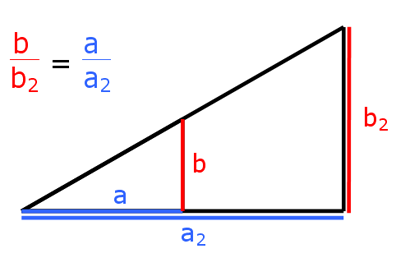
\includegraphics[width=0.35\textwidth]{images/strahlensatz}
\end{center}
\begin{block}{Zentralprojektion}
Die Matrizen
\begin{align*}
K_{persp_{xy}} := \begin{pmatrix}  
1   &  0 & 0 & 0  \\
0   &  1 & 0 & 0  \\
0   &  0 & 1 & 0  \\
0   &  0 & \frac{1}{d} & 0 
\end{pmatrix} ,
K_{orth_{xy}} := \begin{pmatrix}  
1   &  0 & 0 & 0  \\
0   &  1 & 0 & 0  \\
0   &  0 & 0 & 1  
\end{pmatrix} \; ,
\end{align*}
realisieren die Zentralprojektion auf die Ebene parallel zur $X-Y$-Ebene und Augenpunkt im Ursprung mit Augendistanz $d$ in homogenen Koordinaten.


\end{block}
\end{frame}

\begin{frame}
    \frametitle{Perspektive}
\framesubtitle{}
\begin{block}{Zentralprojektion}
Die Zentralprojektion auf die Ebene parallel zur $X-Y$-Ebene und Augenpunkt im Ursprung mit Augendistanz $d$ durch die Hintereinanderausführung folgender Abbildungen darstellen:
\begin{align*}
& persp_{xy} :\mathbb{A}^3   \to \mathbb{P}^3    \to  \mathbb{P}^3    \to \mathbb{P}^2    \to \mathbb{A}^2  \\
&\begin{pmatrix} x \\ y \\ z \end{pmatrix} \mapsto \begin{bmatrix} x \\ y \\ z \\ 1 \end{bmatrix}   \mapsto K_{persp_{xy}} \cdot  \begin{bmatrix} x \\ y \\ z \\ 1 \end{bmatrix} =   \begin{bmatrix} x \\ y \\ z \\ \frac{z}{d}  \end{bmatrix} \\
 & \mapsto K_{orth_{xy}} \cdot   \begin{bmatrix} x \\ y \\ z \\ \frac{z}{d}  \end{bmatrix}=   \begin{bmatrix} x \\ y \\ \frac{z}{d} \end{bmatrix}   \mapsto 
 \begin{pmatrix}  \frac{x}{\frac{z}{d} } \\   \frac{y}{\frac{z}{d} } \end{pmatrix}
 \end{align*}

\end{block}
\end{frame}


\begin{frame}
    \frametitle{Perspektive}
\framesubtitle{}
\begin{block}{Clipping Koordinaten}

\begin{align*}
P := \begin{pmatrix}  
\frac{n}{r}  &  0 & 0  & 0  \\
0   &  \frac{n}{t} & 0 & 0  \\
0   &  0 & \frac{-f-n}{f-n} & \frac{-2\cdot f \cdot n}{f-n}  \\
0   &  0 & -1 & 0  
\end{pmatrix}  \; .
\end{align*} 



\end{block}
\begin{center}
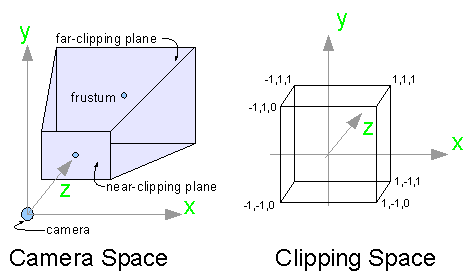
\includegraphics[scale=0.40]{images/projection}
\end{center}
\end{frame}


\begin{frame}
    \frametitle{Perspektive}
\framesubtitle{}
\begin{block}{Projektive Abbildungen}
Wir können mit der Definition der Matrix-Vektor-Multiplikation eine affine Abbildung 
\begin{align*}
\phi : \mathbb{A}^{3} \to \mathbb{A}^{3} \\
\phi(v):=  A \cdot v + t
\end{align*}
in homogenen Koordinate ausdrücken durch eine Matrizenmultiplikation
\begin{align*}
\begin{pmatrix} v \\ 1\end{pmatrix} \mapsto \begin{pmatrix}  A  & t  \\ 0 &1\end{pmatrix} \cdot  \begin{pmatrix} v \\ 1\end{pmatrix}  =    \begin{pmatrix}  A v +t   \\ 1\end{pmatrix}  \; .
\end{align*}
\end{block}
\end{frame}


\begin{frame}
    \frametitle{Perspektive}
\framesubtitle{}
\begin{block}{Projektive Abbildungen}
MVP:= Model View Projection Matrix
\end{block}
\end{frame}



\end{document}
